% \pagebreak[4]
% \hspace*{1cm}
% \pagebreak[4]
% \hspace*{1cm}
% \pagebreak[4]

\chapter{Xây dựng mô hình doc2vec-word2vec trong thực tế}
\ifpdf
    \graphicspath{{Chuong1_hanhbd/Chapter1Figs/PNG/}{Chuong1_hanhbd/Chapter1Figs/PDF/}{Chuong1_hanhbd/Chapter1Figs/}}
\else
    \graphicspath{{Chuong1_hanhbd/Chapter1Figs/EPS/}{Chuong1_hanhbd/Chapter1Figs/}}
\fi

Ngoài các vấn đề cải thiện tốc độ về mặt thuật toán, trong quá trình xây dựng model word2vec  thực tế, ta còn gặp phải các vấn đề như:
\begin{itemize}  

        \item Tính toán với lượng dữ liệu đầu vào lớn

        \item Loại bỏ trùng lặp trong dữ liệu đầu vào

        \item Lọc bỏ các tín hiệu nhiễu, không có giá trị thông tin. \ldots 

    \end{itemize}
    
Ở chương này, tôi sẽ trình bày chi tiết các vấn đề cũng như phương án giải quyết của từng vấn đề trên.  
\section{Tính toán với lượng dữ liệu đầu vào lớn}  \label{DeepDist}

Để đảm bảo một model doc2vec có chất lượng tốt thì số lượng văn bản phải đủ lớn. Tuy nhiên với lượng dữ liệu đầu vào lớn (có thể lên tới hàng triệu thậm chí hàng trăm triệu văn bản) thì việc xây dựng mô hình doc2vec trên 1 máy đơn lẻ sẽ rất tốn thời gian. Một phương pháp dù hoàn hảo đến đầu nếu không thể triển khai thì hoàn toàn vô nghĩa. Vì vậy cần phải có một giải pháp để đảm bảo thời gian xây dựng model trong phạm vi chấp nhận được.

Với sự phát triển của hệ thống điện toán phân tán (Distributed Computing) cũng như sự phổ biến của các công cụ giúp trong việc cấu hình và triển khai các hệ thống phân tán, trong quá trình tìm hiểu tôi nhận thấy vấn đề đặt ra đã được giải quyết sử dụng hệ thống điện toán phân tán và đã được triển khai thành công trên open-source DeepDist \cite{DeepDist} trên nền engine \textsc{Apache Spark}. \cite{ApacheSpark}

Doc2vec trong DeepDist được phát triển trên nền của Gensim \cite{Gensim} - một trong những opensource tốt nhất về về word2vec-doc2vec. DeepDist sử dụng Downpour (tương tự như stochastic gradient descent). Đầu tiên DeepDist khởi tạo tại một máy master. Sau đó, trên mỗi máy slave, DeepDist sẽ lấy model từ master và gọi hàm gradient() và tính toán giống như stochastic gradient descent trên 1 phần dữ liệu .Sau khi tính toán trên các phần dữ liệu này, các thông số cần thiết dùng để cấp nhật trọng số cho model sẽ được gửi lại về master. Lúc này, trên máy master sẽ cập nhật trọng số cho mô hình bằng việc gọi hàm descent(). Quá trình này lặp lại cho đến khi xử lý xong hết toàn bộ các phần dữ liệu, và đảm bảo tính đồng bộ cho các máy slave trong toàn bộ quá trình.

\begin{figure}[!htbp]
  \begin{center}
    %\leavevmode
    \ifpdf
      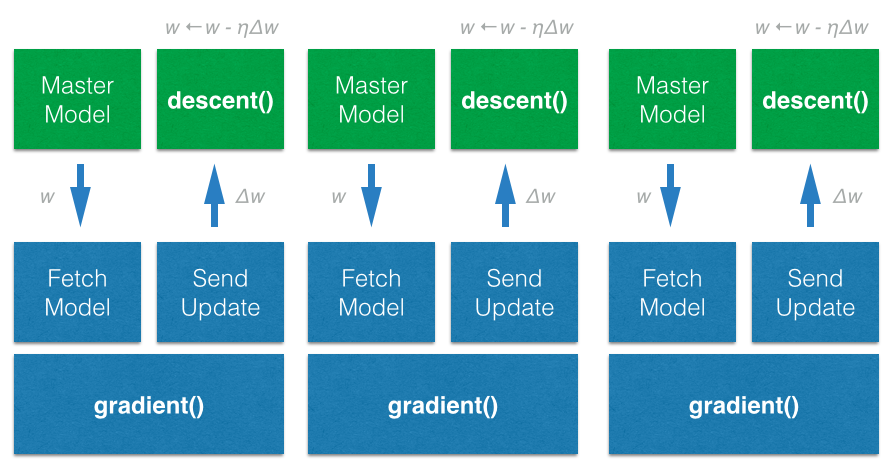
\includegraphics[scale=0.4]{deepdistdesign}
    \else
      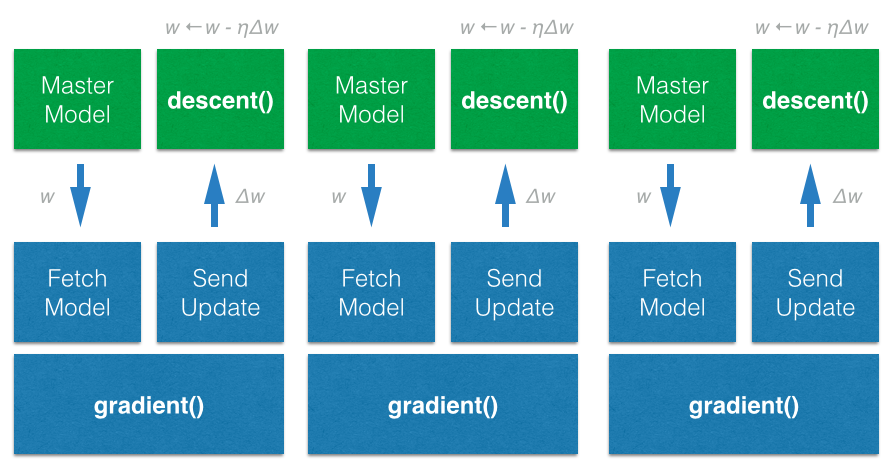
\includegraphics[scale=0.4]{deepdistdesign}
    \fi
    \caption{Mô hình thiết kế của DeepDist}
    \label{deepdistdesign}
  \end{center}
\end{figure}

\section{Loại bỏ trùng lặp trong dữ liệu đầu vào}  

Với đặc trưng dữ liệu đầu vào là các văn bản được crawl về từ mạng internet, dẫn đến việc cần lọc và xử lý các dữ liệu trùng để loại bỏ các đặc trưng ko đáng có cho mô hình là vấn đề vô cùng quan trọng trong quá trình xây dựng model.

Với lượng dữ liệu lớn, việc kiểm tra trùng lặp theo cách đơn thuần là so sánh độ trùng lặp của 2 chuỗi là hoàn toàn bất khả thi từ tài nguyên tính toán đến tốc độ. Vì vậy ta cần một phương án kiểm tra trùng lặp có tính khả thi và thực tế hơn, dù phải chấp nhận hi sinh độ chính xác ở một mức nhất định.

Với mục tiêu "thiếu tốt hơn nhầm" tôi lựa chọn phương án sử dụng giải thuật Bloom-filter vì các đặc trưng sau:
\begin{itemize}  

        \item Độ recall 100\%

        \item Tốc độ kiểm tra $O(1)$

        \item Có thể chủ động được độ false-positives 
        
        \item Tiết kiệm tài nguyên. 

    \end{itemize}
    
\subsection{Mô tả giải thuật}

Một bộ lọc Bloom filter trống là 1 mảng $m$ bit tất cả các bit được set bằng $0$. Ta còn cần định nghĩa $k$ hàm băm trong đó mỗi hàm băm 1 phần tử về 1 vị trí trong mảng bit một cách thống nhất. 

Muốn thêm một phần tử vào bộ lọc, ta chỉ cần băm phần tử đó bằng $k$ hàm hash để lấy ra $k$ vị trí, set bit tại $k$ vị trí này thành $1$.

Muốn kiểm tra một phần tử đã xuất hiện trong bộ lọc hay chưa, ta băm phần tử đó bằng $k$ hàm băm để lấy ra $k$ vị trí và kiểm tra xem có tất cả các bit này có bằng 1 hay không? Nếu đúng thì phần từ đó \textbf{"có thể đã xuất hiện"}. Nếu tồn tại ít nhất 1 bit có giá trị 0 thì phần tử đó \textbf{"chắc chắn chưa xuất hiện"}.

Với yêu cầu là $k$ hàm băm phải độc lập khác nhau nên thuật toán sẽ không thể hoạt động với $k$ quá lớn.
\begin{figure} [!htbp]
  \begin{center}
    %\leavevmode
    \ifpdf
      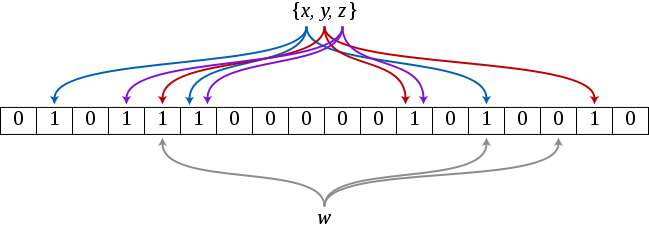
\includegraphics[scale=0.4]{Bloom_filter}
    \else
      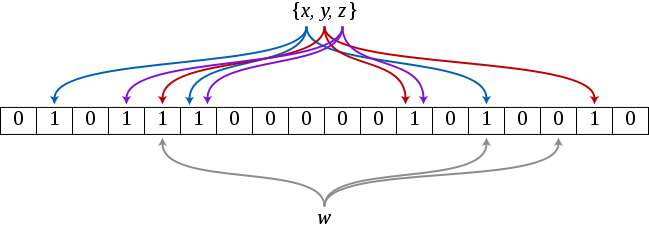
\includegraphics[scale=0.4]{Bloom_filter}
    \fi
    \caption{Ví dụ về Bloom filter với $k=3$ và $m=18$}
    \label{bloomfilter_img}
  \end{center}
\end{figure}

Hình \ref{bloomfilter_img} cho ta ví dụ về một bộ lọc bloom filter với số hàm băm $k =3$ và số bit của mảng là $m = 18$ . Sau khi thêm 3 phần từ $x,y,z$ vào bộ lọc ta kiểm tra $w$ đã thuộc bộ lọc hay chưa. Kết quả trả ra là $w$ không thuộc bộ lọc vì trong 3 bit ứng với $w$ có một bit bằng 0. 

\subsection{False-positives trong Bloom filter}

Tiếp theo ta tìm hiểu về xác suất xuất hiện một kết quả sai hay là một false-posivite trong Bloom-filter.

Giả sử rằng một hàm băm chọn từng vị trí trong mảng với xác suất như nhau. Như vậy, khi thêm một phần tử, xác suất để một bit không được set bằng 1 với một hàm băm là :
\begin{large}
\[ 1 - \dfrac{1}{m}\]
\end{large}

Ta có k hàm băm, như vậy, xác suất để một bit không được set bằng 1 khi thêm một phần tử là :
\begin{large}
\[ {(1 - \dfrac{1}{m})}^{k} \]
\end{large}

Và khi thêm $n$ phần tử, xác suất để một bit không được set bằng 1 là :
\begin{large}
\[ {(1 - \dfrac{1}{m})}^{kn} \]
\end{large}

Như vậy xác suất để một bit được set bằng 1 là :
\begin{large}
\[ 1 - {(1 - \dfrac{1}{m})}^{kn} \]
\end{large}
Giờ ta xét một phần tử không thuộc bộ lọc, xác suất để cả k vị trị được băm ra từ phần từ này đều đã được set bằng 1 là : 
\begin{equation}
{\left( 1 - {\left( 1 - \dfrac{1}{m}\right) }^{kn}\right) }^{k} \approx {\left( 1 - e^{^{-kn}/_{m}}\right)}^{k}
\end{equation}

Nói một cách khác, xác suất để xuất hiện một falsae-positves là :
\begin{equation} \label{false-positive}
P_{err} \approx {\left( 1 - e^{^{-kn}/_{m}}\right)}^{k}
\end{equation}

\subsection{Cấu hình giá trị cho Bloom filter}
Từ (\ref{false-positive}) ta thấy để error rate nhỏ nhất thì 
\begin{equation} \label{khash}
k = \dfrac{m}{n} \ln{2}
\end{equation}

Tuy nhiên thực tế thì số lượng hàm băm là nhỏ và chỉ có một mức cụ thể. Thay giá trị trên ngược về (\ref{false-positive}) ta có : 
\begin{equation} \label{perror}
\ln{p} = - \dfrac{m}{n} (\ln{2})^2
\end{equation}
\begin{equation} \label{mbit}
m = - \dfrac{n\ln{p}}{(\ln{2})^2} 
\end{equation}

Như vậy, thay vì truyền vào $m, k$ và tính toán ra giá trị của $n$ và $p$ thì ta hoàn toàn có thể truyền vào $n,p$ là những thông số ta dễ ước lượng cũng như mong muốn và tính toán các giá trị còn lại thông qua (\ref{khash}) và (\ref{mbit}). 

\subsection{Ứng dụng Bloom filter trong lọc trùng văn bản}

Do đặc tính của hàm băm nên với một văn bản, chỉ cần một chút thay đổi nhỏ về dấu, người viết,... là đã được một văn bản có giá trị băm hoàn toàn khác trong khi nội dung chính lại giống nhau hoàn toàn. 

Vì vậy tôi lựa chọn giải pháp coi văn bản là tập hợp các câu. Việc đánh giá một văn bản đã tồn tại trong bộ lọc hay chưa sẽ phù thuộc vào số câu của nó đã xuất hiện trong bộ lọc hay chưa. Nếu tỷ lệ số câu đã xuất hiện trong bộ lọc trên tổng số câu của văn bản vượt qua một ngưỡng xác định thì ta coi như văn bản này đã xuất hiện. Tất nhiên điều này khiến cho độ chính xác cũng như việc ước lượng chính xác số phần tử trong bộ lọc trở nên khó khăn hơn, nhưng xét trên mục đích "thiếu còn hơn thừa" thì điều này có thể chấp nhận được.